\chapter{Correzione, sviluppo e ottimizzazione Demo A} \label{ch:DemoA}

All'interno di questo capitolo sarà fornita una descrizione completa dei lavori svolti nel primo progetto di demo che è stato preso in analisi inizialmente, corretto e migliorato successivamente.
\\ Inizialmente viene descritta con una breve introduzione gli obiettivi che ci si aspettava di raggiungere con lo sviluppo della demo, i problemi presenti all'inizio del lavoro svolto e le soluzioni possibili attuabili.
\\ Nella seconda parte viene trattato, entrando più nello specifico, l'implementazioni delle soluzioni proposte e presentato il lavoro finale. 
\\ Nell'ultima parte del capitolo viene infine mostrato una prova di correttezza della demo con la verifica dei suoi output e delle sue funzionalità.


\section{Introduzione alla Demo}
Come descritto al Capitolo[\ref{ch:verefoo}] Verefoo è un framework in grado di definire dei requisiti di sicurezza ad alto livello, allocare in maniera ottimale varie Network Security Functions (NSF) all'interno della topologia di rete fornita in input e configurare automaticamente tali funzioni 
automaticamente. Allo stato attuale il framework è ancora in fase di sviluppo e, nonostante si ponga gli obiettivi appena descritti, non tutte le funzionalità sono attualmente possibili all'interno del framework. Più precisamente, varie versioni del framework sono presenti in stato di sviluppo, e ognuna si occupa di allocare una possibile NSF separatamente alle altre.
All'interno di questo capitolo verrà presa in considerazione per il lavoro una di queste possibili versioni, ovvero quella che si occupa della verifica dei Network Security Requirements di protezione, dell'allocazione del numero minimo ottimale di VPN Gateway per rispettare i requisiti in input, e della configurazione di questi ultimi.\\
L'obiettivo principale di questo lavoro di demo è quindi mostrare all'utente come questa versione sia in grado, data una topologia di rete simile a quelle di una azienda di medie dimensioni, di verificare i requisiti, allocare le VPN e configurarle correttamente.
\newpage
Un altro elemento emerso durante i lavori sullo sviluppo di questa demo è stata la difficile accessibilità di quest'ultima. Per far funzionare sia il framework che la demo sono infatti necessari numerosi tool da installare all'interno della macchina in alcune versioni specifiche e potrebbe essere non immediato installare correttamente il dispositivo per far funzionare 
framework e demo. Di conseguenza come obiettivo secondario, ma di uguale importanza è stato prodotto un installer che permette all'utente di ottenere automaticamente tutti i programmi nelle versioni corrette per poter utilizzare il framework a proprio piacimento.
\\
Per portare a termine questi due obiettivi ci si è quindi interfacciati con un progetto di demo che risultava incompleto e mal funzionante. Analizzando più approfonditamente possiamo dividere le modifiche effettuate all'interno di questa demo nei seguenti punti:

\begin{enumerate}
    \item \textbf{Versione Framework}: Il file del framework iniziale era malfunzionante, in quanto ogni qual volta che si provava ad avviarlo il terminale segnalava il file come corrotto ed inutilizzabile.
    \item \textbf{Chiamate API}: La demo utilizzava delle chiamate API considerabili obsolete, di conseguenza qualsiasi relazione con il framework non produceva alcun risultato.
    \item \textbf{Installer}: Come accennato precedentemente la mancanza di un installer della Demo rendeva il framework poco accessibile e di difficile installazione manuale.
    \item \textbf{Certificati VPN}: Alcuni dei certificati di chiavi pubbliche e private erano ormai scaduti, sono quindi stati sostituiti ed i file di configurazione modificati opportunatamente.
    \item \textbf{Docker Compose}: Il file di configurazione dell'ambiente virtuale di Docker Compose conteneva errori e molti dei container non venivano istanziati correttamente.
    \item \textbf{Forwarding Rules}: Alcune forwarding rules all'interno dell'ambiente virtuale erano scorrette, sono state quindi corrette ed aggiornate per garantire la comunicazione fra tutti i nodi della rete.
\end{enumerate}

    
\section{Implementazione}
Welcome to the demo of Verefoo for VPNs. What you will see written here will be a simple stand-alone demo in which the features and capabilities of Verefoo are highlighted.
Before we begin we need to define a network topology that Verefoo will need to relate to, more precisely you will also need to define the respective IP addresses and links between the different nodes.  During the course of the demo, a virtual environment developed with Docker Containers will be instantiated that will reproduce the topology presented in this document.

\begin{figure}[h]  % 'h' significa che la figura viene posizionata qui
    \centering
    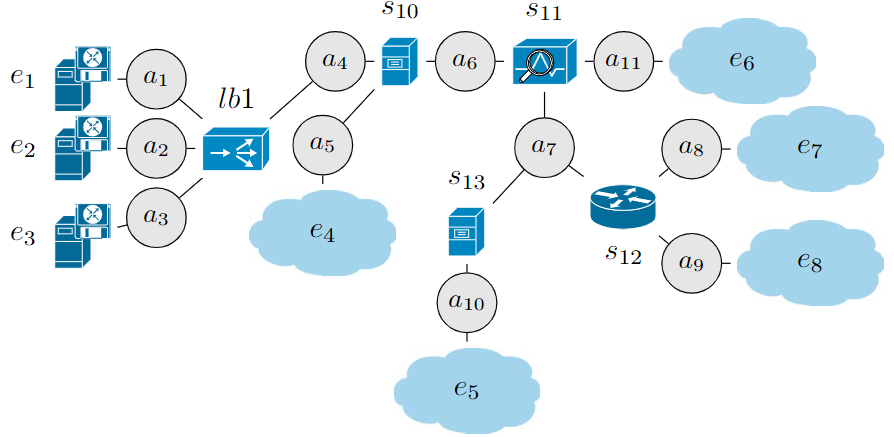
\includegraphics[width=1\textwidth]{VPN_AG.PNG} 
    \caption{Service Graph}
    \label{fig:ServiceGraph}
\end{figure}
As can be seen, the proposed topology has 3 webservers on the left whose traffic is handled by a load balancer and 5 endpoints that are represented by web clients. Within the network there are nodes that will act as monitors, such as node s11, and others that will instead perform the simple forwarder function with their respective static routes. Finally, there are several currently empty nodes that we will call allocation places. Within these nodes, the framework will be able to place network security functions to make sure that the security requirements are working properly within the network. A table is provided below with the definition of each node, its IP address that will be used in the virtual environment, and its functionality within the topology.

\begin{table}[h]
    \centering
    \begin{tabular}{ccc}
        \hline
         Name & IP & Functionality \\
        \hline
        e1 & 130.10.0.1 & Web servers behind load balancer b1 \\
        e2 & 130.10.0.2 & * \\
        e3 & 130.10.0.* & * \\
        e4 & 40.40.41.* & Web Client \\ 
        e5 & 40.40.41.* & Web Client \\
        e6 & 88.80.84.* & Web Client \\
        e7 & 192.168.1.* & Web Client \\
        e8 & 192.168.2.* & Web Client \\
        lb1 & 130.10.0.4 & Load Balancer \\
        s10 & 33.33.33.2 & Web Cache \\
        s11 & 33.33.33.3 & Forwarder \\
        s12 & 220.124.30.1 & Forwarder \\
        s13 & 33.33.33.4 & Forwarder \\
        a7 & 1.0.0.7 & Forwarder \\
        \hline
    \end{tabular}
    \caption{Node definitions and functionalities}
    \label{tab:tabella}
\end{table}


The second and final input that must be provided to the framework is the set of security requirements that the network must have. With this demo, the goal was to have an output topology that contained a large number of VPN Gateways (6), in order to be able to show an example that would come as close as possible to a hypothetical real case of a small-to-medium sized company. In order to be able to achieve a similar topology, the following rules were defined:
\\
\\

\begin{table}[h]
    \centering
    \small
    \begin{tabular}{ccccccccc}
        \hline
         Policy & IPSrc & IPDst & pSrc & pDst & tProto & Confidentiality & Intregrity & Untrusted nodes\\
        \hline
        Protection & 40.40.41.1 & 130.10.0.1 & * & 22 & ANY & AES-256-CBC & SHA2-256 & 33.33.33.2 \\
        Protection & 88.80.84.1 & 130.10.0.* & * & 80 & ANY & AES-256-CBC & SHA2-256 & 33.33.33.2/33.33.33.3 \\
        Protection & 192.168.1.1 & 130.10.0.1 & * & * & ANY & AES-256-CBC & SHA2-256 & 33.33.33.2/33.33.33.3 \\
        Protection & 40.40.42.1 & 192.168.2.1 & * & * & ANY & AES-256-CBC & SHA2-256 & 33.33.33.4/220.124.30.1 \\
        \hline
    \end{tabular}
    \caption{Security Requirements Definition}
    \label{tab:tabella}
\end{table}
\begin{itemize}
    \item \textbf{First Rule}: Web Client e4 must be able to communicate securely with Web Server e1. Traffic originating from e4 can use any port for the transport protocol but the e5 Server must receive data only from port 22. Both UDP and TCP protocols can be used for communications. Finally, node s10 is specified as a non-secure node and through which traffic must pass encrypted.
    \item \textbf{Second Rule}: Web Client e8 must be able to communicate securely with all Web Servers (e1,e2,e3). Traffic originating from e8 can use any port for the transport protocol but the servers must receive data only from port 80. It is possible to use either UDP or TCP protocol for communication. In this case the nodes that are considered non-secure are s10 and s11.
    \item \textbf{Third Rule}: Web Client e7 must be able to communicate securely with Web Server e1. There are no limitations on ports for incoming and outgoing traffic, and any fourth-level protocol can be used. The unsecured nodes, as with the second rule, are s10 and s11. 
    \item \textbf{Fourth Rule}:The Web Client e5 must be able to communicate securely with the Web Client e8. As with the third rule, there are no limitations on the ports and transport protocol to be used. The nodes considered insecure for this rule are s12 and s13.
\end{itemize}

\section{Output}
By providing the previously defined inputs, the framework will look for a solution that not only satisfies all the rules, but also employs the least amount of resources necessary to guarantee these properties. Verefoo will then solve a problem defined as MaxSMT (Maximum Satisfiability Modulo Theories). 
In the specific case of this demo, the result produced in output will be as follows:

\begin{figure}[h]  % 'h' significa che la figura viene posizionata qui
    \centering
    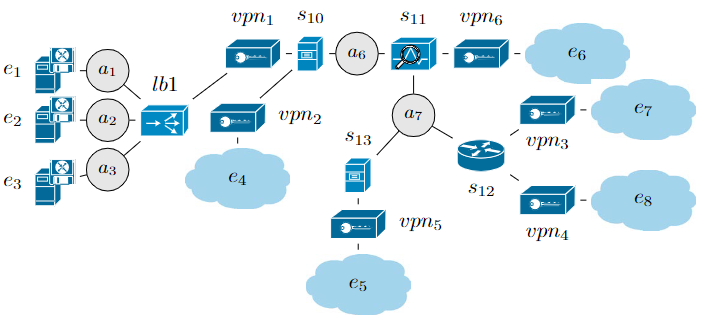
\includegraphics[width=1\textwidth]{VPN_deploy.PNG} 
    \caption{Verefoo Output}
    \label{fig:VPNDeploy}
\end{figure}

As could be imagined, several VPN Gateways were allocated in place of the various Allocation Places defined in the input provided to Verefoo. Given this should be the solution to the problem defined earlier, we will try to test inside the virtual environment the functionality of the various VPN tunnels to make sure that the framework works properly.
Before proceeding, however, it is also important to analyze the various elements that Verefoo has produced. In fact, the framework not only allocates the gateways in the correct places, but also provides an automatic configuration to use. In this specific case, the configuration is as follows:
\\

\begin{table}[ht]
    \centering
    \begin{tabular}{ccccccc}
        \hline
         \# & Action & IPSrc & IPDst & pSrc & pDst & tProto \\
        \hline
        1 & EXIT & 192.168.1.1 & 130.10.0.1 & * & * & ANY \\
        2 & EXIT & 88.80.84.1 & 130.10.0.3 & * & 80 & ANY \\
        3 & EXIT & 40.40.41.1 & 130.10.0.1 & * & 22 & ANY \\
        4 & EXIT & 88.80.84.1 & 130.10.0.1 & * & 80 & ANY \\
        5 & EXIT & 88.80.84.1 & 130.10.0.2 & * & 80 & ANY \\
        6 & ACCESS & 130.10.0.1 & 192.168.1.1 & * & * & ANY \\
        7 & ACCESS & 130.10.0.3 & 88.80.84.1 & 80 & * & ANY \\
        8 & ACCESS & 130.10.0.1 & 40.40.41.1 & 22 & * & ANY \\
        9 & ACCESS & 130.10.0.1 & 88.80.84.1 & 80 & * & ANY \\
        10 & ACCESS & 130.10.0.2 & 88.80.84.1 & 80 & * & ANY\\
        \hline
    \end{tabular}
    \caption{VPN Gateway 1}
    \label{tab:VPN Gateway 1}
\end{table}

\begin{table}[ht]
    \centering
    \begin{tabular}{ccccccc}
        \hline
         \# & Action & IPSrc & IPDst & pSrc & pDst & tProto \\
        \hline
        1 & ACCESS & 40.40.41.1 & 130.10.0.1 & * & 22 & ANY \\
        2 & EXIT & 130.10.0.1 & 40.40.41.1 & 22 & * & ANY \\
        \hline
    \end{tabular}
    \caption{VPN Gateway 2}
    \label{tab:VPN Gateway 2}
\end{table}

\begin{table}[H]
    \centering
    \begin{tabular}{ccccccc}
        \hline
         \# & Action & IPSrc & IPDst & pSrc & pDst & tProto \\
        \hline
        1 & ACCESS & 192.168.1.1 & 130.10.0.1 & * & * & ANY \\
        2 & EXIT & 130.10.0.1 & 192.168.1.1 & * & * & ANY \\
        \hline
    \end{tabular}
    \caption{VPN Gateway 3}
    \label{tab:VPN Gateway 3}
\end{table}

\begin{table}[H]
    \centering
    \begin{tabular}{ccccccc}
        \hline
         \# & Action & IPSrc & IPDst & pSrc & pDst & tProto \\
        \hline
        1 & ACCESS & 192.168.2.1 & 40.40.42.1 & * & * & ANY \\
        2 & EXIT & 40.40.42.1 & 192.168.2.1 & * & * & ANY \\
        \hline
    \end{tabular}
    \caption{VPN Gateway 4}
    \label{tab:VPN Gateway 4}
\end{table}

\begin{table}[H]
    \centering
    \begin{tabular}{ccccccc}
        \hline
         \# & Action & IPSrc & IPDst & pSrc & pDst & tProto \\
        \hline
        1 & ACCESS & 40.40.42.1 & 192.168.2.1 & * & * & ANY \\
        2 & EXIT & 192.168.2.1 & 40.40.42.1 & * & * & ANY \\
        \hline
    \end{tabular}
    \caption{VPN Gateway 5}
    \label{tab:VPN Gateway 5}
\end{table}

\begin{table}[H]
    \centering
    \begin{tabular}{ccccccc}
        \hline
         \# & Action & IPSrc & IPDst & pSrc & pDst & tProto \\
        \hline
        1 & ACCESS & 88.80.84.1 & 130.10.0.1 & * & 80 & ANY \\
        2 & ACCESS & 88.80.84.1 & 130.10.0.2 & * & 80 & ANY \\
        3 & ACCESS & 88.80.84.1 & 130.10.0.3 & * & 80 & ANY \\
        4 & EXIT & 130.10.0.1 & 88.80.84.1 & 80 & * & ANY \\
        5 & EXIT & 130.10.0.2 & 88.80.84.1 & 80 & * & ANY \\
        6 & EXIT & 130.10.0.3 & 88.80.84.1 & 80 & * & ANY \\
        \hline
    \end{tabular}
    \caption{VPN Gateway 6}
    \label{tab:VPN Gateway 6}
\end{table}

\section{Verifiche e Test}